\section{Impact of FASER$\nu$ Run III measurements}
\label{app:fasernu_runIII_impact}


%
Fig.~\ref{fig:profiling_FASERv2_vs_FASERv} shows a comparison of the impact 
that FASER$\nu$2 and FASER$\nu$ pseudodata have in PDF profiling, illustrating 
the improvement in precision obtainable with FASER$\nu$2.

%%%%%%%%%%%%%%%%%%%%%%%%%%%%%%%%%%%%%%%%%%%%%%%%%%%%%%%%%%
\begin{figure}[t]
\centering
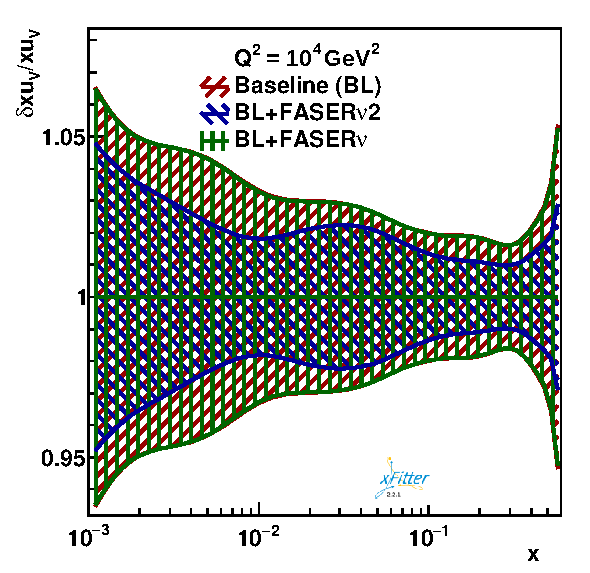
\includegraphics[width=0.32\textwidth]{plots/proton_fasernu2/FASERv2_vs_FASERv/statOnly_FASERv_q2_10000_pdf_uv_ratio.pdf}
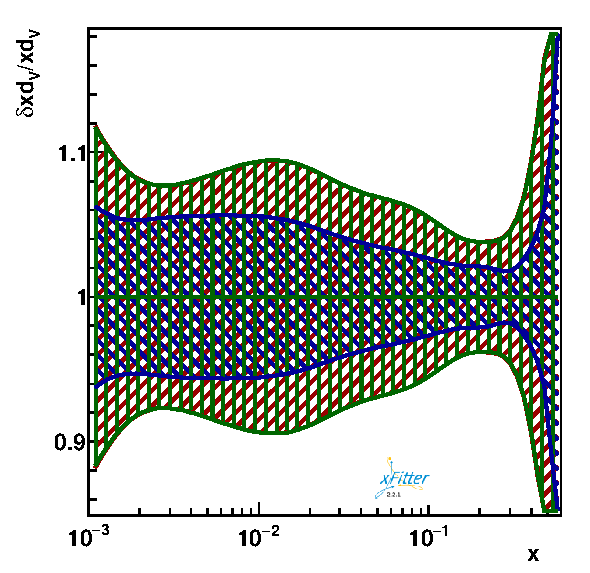
\includegraphics[width=0.32\textwidth]{plots/proton_fasernu2/FASERv2_vs_FASERv/statOnly_FASERv_q2_10000_pdf_dv_ratio.pdf}
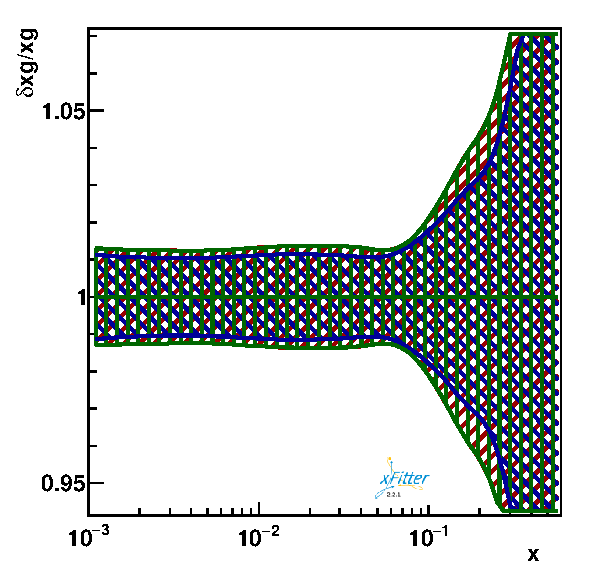
\includegraphics[width=0.32\textwidth]{plots/proton_fasernu2/FASERv2_vs_FASERv/statOnly_FASERv_q2_10000_pdf_g_ratio.pdf}\\
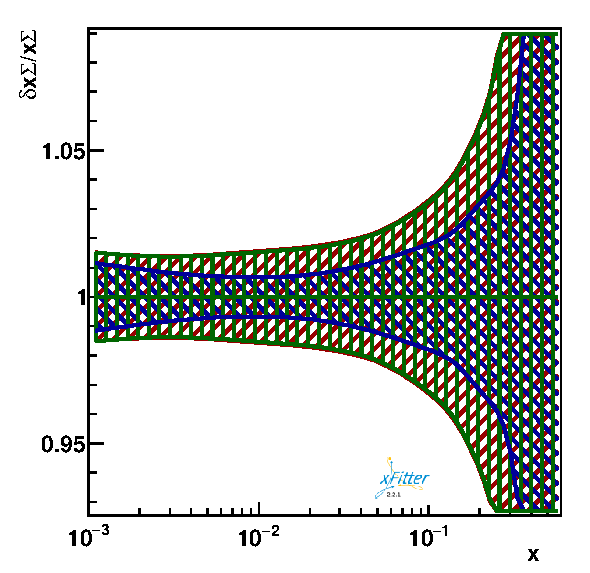
\includegraphics[width=0.32\textwidth]{plots/proton_fasernu2/FASERv2_vs_FASERv/statOnly_FASERv_q2_10000_pdf_Sea_ratio.pdf}
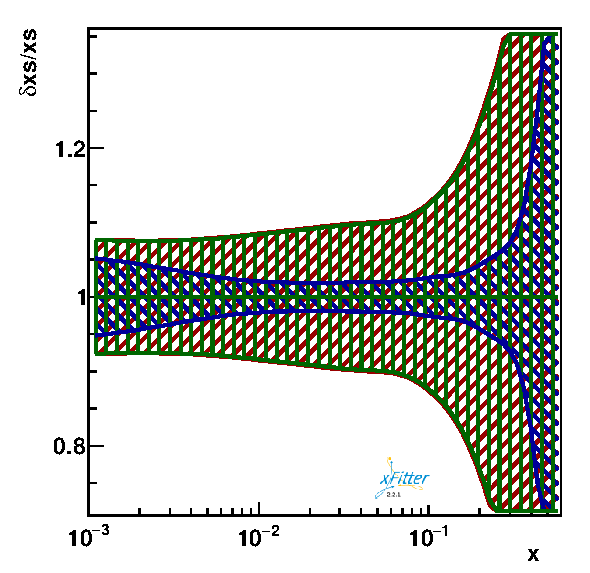
\includegraphics[width=0.32\textwidth]{plots/proton_fasernu2/FASERv2_vs_FASERv/statOnly_FASERv_q2_10000_pdf_s_ratio.pdf}
\caption{
A comparison of the effect of FASER$\nu$ and FASER$\nu2$ pseudodata in profiling, 
assuming only statistical uncertainties in the case of both experiments.
}
\label{fig:profiling_FASERv2_vs_FASERv}
\end{figure}
%%%%%%%%%%%%%%%%%%%%%%%%%%%%%%%%%%%%%%%%%%%%%%%%%%%%%%%%%%%
